\section{Information Geometry of Learning: Fisher Metrics, Natural Gradients,
and Prior Selection}
\label{sec:info-geo}

The machinery of Section~\ref{sec:capabilities} computes, for every learned
model, the gradient of a loss with respect to its parameters and then takes a
step. \emph{Which} step is taken --- AdamW or L-BFGS --- is a computational
choice; \emph{where} the step points is a geometric fact. This section
records the geometry we have adopted as the conceptual background for
\texttt{thotgrad} and \texttt{thotopt}. A parametric family of models is a
curved space of probability distributions; the Fisher information matrix is
its Riemannian metric; the natural gradient is the corresponding steepest
descent \cite{amari1998,amari1985}; and --- following Snoussi's manuscript on
prior selection on
statistical manifolds --- the prior itself is best understood as a density on
that same space, obtained by variational calculus and placed by projection.
In one sentence: information geometry tells a learning system not only
\emph{how} to optimise, but also \emph{where} to place its beliefs before any
data arrives.

\begin{figure}[h]
\centering
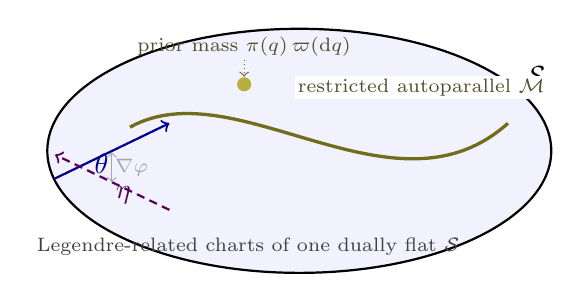
\begin{tikzpicture}[scale=1.0]
  % the statistical manifold as a charted space
  \draw[thick,fill=blue!5] (3,0) ellipse (3.2 and 1.55);
  \node at (6.0,0.95) {$\mathcal S$};
  % natural and dual coordinates (two charts, one manifold)
  \draw[->,thick,blue!55!black] (-0.1,-0.35) -- (1.35,0.35)
        node[midway,below left=0pt,inner sep=1pt] {$\theta$};
  \draw[->,thick,violet!70!black,densely dashed] (1.35,-0.75) -- (-0.1,-0.05)
        node[midway,below right=0pt,inner sep=1pt] {$\eta$};
  % Legendre bridge between the charts
  \draw[<->,gray!70] (0.62,-0.02) -- (0.62,-0.40)
        node[midway,right=0pt,inner sep=1pt,font=\scriptsize]
        {$\nabla\varphi$};
  \node[font=\scriptsize,gray!50!black] at (2.35,-1.22)
        {Legendre-related charts of one dually flat $\mathcal S$};
  % restricted autoparallel submanifold carrying the prior mass
  \draw[very thick,olive!75!black] (0.85,0.30)
        .. controls (2.2,1.05) and (4.2,-0.95) .. (5.65,0.35);
  \node[circle,fill=olive!65,inner sep=1.8pt] (q) at (2.3,0.845) {};
  \node[font=\scriptsize,olive!45!black] at (2.3,1.32)
        {prior mass $\pi(q)\,\varpi(\mathrm{d}q)$};
  \draw[->,olive!60!black,densely dotted] (2.3,1.15) -- (q);
  \node[font=\scriptsize,olive!45!black,fill=white,inner sep=1pt] at (4.55,0.80)
        {restricted autoparallel $\mathcal M$};
\end{tikzpicture}
\caption{The geometry adopted in this section, schematically.  A parametric
family $\mathcal S$ is a statistical manifold carrying two Legendre-related
charts: natural coordinates $\theta$ and expectation coordinates $\eta$;
dually flat means both affine charts are simultaneously flat.  Prior
selection (Snoussi) is the variational placement of a prior mass
$\pi(q)\,\varpi(\mathrm{d}q)$ on a restricted autoparallel submanifold
$\mathcal M$ --- the belief-corridor of
Section~\protect\ref{sec:info-geo-prior}.}
\label{fig:info-geo-schematic}
\end{figure}

\subsection{Statistical Manifolds and the Fisher Metric}
\label{sec:info-geo-fisher}

Consider a family of probability distributions
$p_\theta(y\mid x)$, $\theta \in \Theta \subseteq \R^{n}$, large enough that
different $\theta$ describe perceptibly different behaviour. The family is a
\emph{statistical manifold}: the point $p_\theta$ corresponds to a full
conditional distribution (a model over outcomes), the coordinates $\theta$ are
a chart on it, and learning --- estimating $\theta$ from data, or updating a
belief over $\theta$ --- is motion on this space rather than on an arbitrary
Euclidean parametrisation of it. The distance that makes this statement
precise is the Kullback--Leibler divergence, and its local form is quadratic.
For a regular family one has
\begin{equation}
d_{\mathrm{KL}}\!\left(p_\theta \,\|\, p_{\theta + d\theta}\right)
\;=\; \tfrac{1}{2}\, d\theta^{\top} F(\theta)\, d\theta
    + \mathcal{O}(\lVert d\theta \rVert^{3}),
\qquad
F_{ij}(\theta) \;=\;
\E_\theta\!\left[\partial_i \log p_\theta \,\cdot \partial_j \log p_\theta\right]
\label{eq:geo-kl}
\end{equation}
with $F$ the \emph{Fisher information matrix} (equivalently
$F_{ij} = -\,\E_\theta\!\left[\partial_i \partial_j \log p_\theta\right]$ when
the derivative may be taken under the expectation). Divergences are not
metrics in general, but for infinitesimally separated points the KL
divergence \emph{is} a squared distance, and $F$ --- the pullback of that
quadratic form to the parameter chart --- behaves exactly like a Riemannian
metric: it transforms with the square of the Jacobian under
reparametrisation and is positive semidefinite, with degenerate directions
corresponding to non-identified parameters. A classical uniqueness result of
Chentsov \cite{chentsov1972} goes further: the Fisher metric is, up to
monotone rescaling, the
only Riemannian metric on a family of distributions that is invariant under
all reasonable transformations of the data (roughly, under randomised
post-processing that preserves sufficient statistics). The geometry is not a
choice; it is forced by what statistics is allowed to do.

The Fisher metric is only the first half of the structure. On families of
exponential (and of mixture) type, Amari's information geometry
\cite{amari1985} associates to
the model a one-parameter family of $\alpha$-connections; in the
$\delta$-labelling used by Snoussi one works with the dual pair
$\nabla^{\delta}$, $\nabla^{1-\delta}$, which are mutually dual with respect
to the Fisher metric:
$\partial_Z\langle X, Y\rangle = \langle \nabla_Z X, Y\rangle
+ \langle X, \nabla^{*}_Z Y\rangle$ for tangent fields $X, Y, Z$. When either
connection is flat the manifold is \emph{dually flat} and carries two
privileged coordinate systems related by a Legendre transform,
\begin{equation}
\frac{\partial \psi}{\partial \theta_i} = \eta_i,
\qquad
\frac{\partial \varphi}{\partial \eta_i} = \theta_i,
\qquad
\frac{\partial \eta_j}{\partial \theta_i} = F_{ij},
\label{eq:geo-legendre}
\end{equation}
with $\psi, \varphi$ dual convex potentials. In the two flat limits these are
the natural (log-partition-type) parameters $\theta$ of the exponential
family and the dual expectation (mean/mixture) parameters $\eta$: straight
lines in $\theta$-coordinates are exponential arcs, straight lines in
$\eta$-coordinates are mixture arcs, and Young-duality exchanges the two
charts. This is the famous dualistic structure $(F, \nabla, \nabla^{*})$ of
Amari's information geometry, and it is the reason several inferential
objects (orthogonal projection, best approximation, fixed points
of the em algorithm) come in dual pairs.

The metric turns the loss landscape into a Riemannian problem, and steepest
descent on a Riemannian manifold is not the plain gradient in coordinates:
steepest descent follows $-F^{-1}\nabla\mathcal{L}$. Concretely, the
\emph{natural-gradient} update is
\begin{equation}
\theta \;\leftarrow\; \theta \;-\; \eta\, F(\theta)^{-1}\, \nabla_\theta\,
\mathcal{L}(\theta),
\label{eq:geo-ng}
\end{equation}
i.e.\ Euclidean steepest descent pre-conditioned by the inverse Fisher
matrix, or equivalently descent in KL distance rather than in parameter norm.
Where $F$ is singular the update is ill-defined along the kernel
directions --- the same non-identifiability that Snoussi's prior analysis
(below) cures by regularisation. The decisive property of \eqref{eq:geo-ng} is its
coordinate-independence:

\begin{theorem}[Parameterisation invariance of the natural gradient]
\label{thm:ng-invariance}
Let $\theta' = \phi(\theta)$ be a diffeomorphism with non-singular Jacobian
$\mathrm{J} = \partial\theta/\partial\theta'$, and suppose the losses
$\mathcal{L}(\theta)$ and $\mathcal{L}'(\theta')$ are coordinate expressions
of one and the same scalar function on the manifold. Then the natural-gradient
step transforms as the corresponding displacement,
\[
\Delta\theta' = \left(\tfrac{\partial\theta'}{\partial\theta}\right)
\Delta\theta = \mathrm{J}^{-1}\,\Delta\theta,
\qquad
\Delta\theta = -\eta\,F^{-1}\nabla_\theta\mathcal{L},
\quad
\Delta\theta' = -\eta\,F'^{-1}\nabla_{\theta'}\mathcal{L}',
\]
whereas the plain gradient step $\Delta\theta' = -\eta\,\nabla_{\theta'}
\mathcal{L}'$ does not obey this displacement law.
\end{theorem}

\begin{proof}
Chain rule under the invariant expectation gives
$\nabla_{\theta'}\mathcal{L}' = \mathrm{J}^{\top}\nabla_\theta\mathcal{L}$ and
$F' = \mathrm{J}^{\top} F\, \mathrm{J}$, so that
\[
-\eta\,F'^{-1}\nabla_{\theta'}\mathcal{L}'
= -\eta\,(\mathrm{J}^{\top}F\mathrm{J})^{-1}\mathrm{J}^{\top}
\nabla_\theta\mathcal{L}
= \mathrm{J}^{-1}\,\bigl(-\eta\,F^{-1}\nabla_\theta\mathcal{L}\bigr)
= \mathrm{J}^{-1}\,\Delta\theta,
\]
which is exactly the tangent-vector transformation law for a displacement
between the two charts. The plain gradient step transforms with
$\mathrm{J}^{\top}$ instead of $\mathrm{J}^{-1}$; the two agree only for
orthogonal changes of scale, so plain gradient descent manufactures different
trajectories in different coordinates for the same modelling problem.
\end{proof}

\begin{remark}
Theorem~\ref{thm:ng-invariance} is the operational content of ``the Fisher
matrix is the metric'': plain gradient descent measures distance with a
metric that changes under relabelling of coordinates, the natural gradient
descends the same loss in KL distance whatever chart is used. Amari
emphasised this as the reason natural-gradient learning is simultaneously
better conditioned and better defined --- it is the geodesic intuition,
translated into an update rule.
\end{remark}

\subsection{Placing Beliefs on a Statistical Manifold: Snoussi's Variational
Prior}
\label{sec:info-geo-prior}

Everything above concerns \emph{how} to move on the manifold. The second
question --- \emph{where to place a belief before data arrives} --- is the
subject of the manuscript \emph{Bayesian Information Geometry: Application to
Prior Selection on Statistical Manifolds} by H.~Snoussi (University of
Technology of Troyes) \cite{snoussi2007}, which we summarise here because it
shaped how we think
about the probabilistic parts of the pipeline. Its setting is deliberately
general: given a statistical manifold $\mathcal{Q}$ of distributions (the
computationally tractable parametric model, embedded in the space of all
probability measures), a Bayesian decision rule maps data to a point of
$\mathcal{Q}$; a prior is nothing but a probability density $\Pi(\theta)$
\emph{on the manifold itself}, a mass spread over the points $p_\theta$.
Snoussi's observation is that prior selection is the \emph{inverse problem}
of statistical learning: instead of fixing a prior and finding the optimal
decision (the barycentre of the posterior mass), one fixes the optimal
decision --- an expert-supplied reference distribution $p_0$ representing
\emph{the weights the system would wager without data} --- and asks which
mass $\Pi$ would have produced it. The chosen decision must be honest
(exclusive concentration on $p_0$ would smuggle in knowledge) and uniform
(no irrelevant information); these two demands are traded off explicitly.
In the $\delta$-geometry on the space of distributions --- generated by the
$\delta$-divergence family
% (Snoussi eq.~(6); his stated identity D_1(p,q) = D_0(q,p) = KL(p||q) holds
% under this exponent placement, verified numerically against the sources.)
\begin{equation}
D_\delta(p, q) = \frac{1}{\delta(1-\delta)}
\int \bigl[\,\delta\,p + (1-\delta)\,q
- p^{\delta}\,q^{\,1-\delta}\,\bigr] d\mu
\quad(\delta \in (0,1)),
\qquad
D_1(p,q) = D_0(q,p) = d_{\mathrm{KL}}(p\,\|\,q),
\label{eq:geo-divergence}
\end{equation}
with $\mu$ a dominant measure on the data space --- and an $\alpha$-geometry
on the space of priors, the cost to minimise is
\begin{equation}
J_{\delta,\alpha}(\Pi) \;=\;
\gamma_e \int \Pi(\theta)\, D_\delta(p_\theta,\, p_0)\, d\theta
\;+\;
\gamma_u\, D_\alpha\bigl(\Pi,\; \sqrt{g}\bigr),
\label{eq:geo-cost}
\end{equation}
where $\sqrt{g}(\theta) = \sqrt{\det F(\theta)}$ is the Jeffreys density ---
the uniform measure \emph{of the statistical manifold}, which by its
invariance represents ignorance better than any coordinate-wise uniform
density --- and the weights $\gamma_e, \gamma_u$ encode confidence in the
reference and the degree of required uniformity, respectively.

\begin{proposition}[The $(\delta,\alpha)$-prior; Snoussi, Thm.~1]
\label{prop:snoussi-prior}
The minimiser of $J_{\delta,\alpha}$ \eqref{eq:geo-cost} over the densities
$\Pi$ is, for $\alpha \neq 1$,
\begin{equation}
\Pi_{\delta,\alpha}(\theta) \;\propto\;
\frac{\sqrt{g(\theta)}}
{\bigl[\,1 + (1-\alpha)\,\tfrac{\gamma_e}{\gamma_u}
\,D_\delta(p_\theta,\, p_0)\bigr]^{1/(1-\alpha)}},
\qquad
\Pi_{\delta}(\theta) \;\propto\;
e^{-\frac{\gamma_e}{\gamma_u} D_\delta(p_\theta,\,p_0)}\,\sqrt{g(\theta)}
\quad(\alpha = 1).
\label{eq:geo-prior}
\end{equation}
\end{proposition}

\begin{proof}
The first variation of \eqref{eq:geo-cost}, computed by the variational
calculus (with $D_\alpha$ acting on the density ratio $\Pi/\sqrt{g}$), is
proportional to
$\int \delta\Pi(\theta)\,\bigl[\gamma_e D_\delta(p_\theta,p_0)
+ \tfrac{\gamma_u}{1-\alpha}\bigl(1-(\Pi/\sqrt{g})^{\alpha-1}\bigr)\bigr]
\,d\theta$ for $\alpha \neq 1$, and to
$\int \delta\Pi\,\bigl[\gamma_e D_\delta(p_\theta,p_0)
+ \gamma_u \log(\Pi/\sqrt{g})\bigr]\,d\theta$ for $\alpha = 1$.
Setting each bracket to zero recovers \eqref{eq:geo-prior}, using
$(\Pi/\sqrt{g})^{\alpha-1}
= 1 + (1-\alpha)\tfrac{\gamma_e}{\gamma_u}D_\delta$ in the first case and
exponentiating in the second.
\end{proof}

The family \eqref{eq:geo-prior} interpolates coherently between the classical
non-informative priors as the geometry and the confidence ratio vary:
\begin{itemize}
    \item $(\delta,\alpha) = (1,1)$: the Kullback--Leibler case; the prior is
          the \emph{entropic} prior.
    \item $(\delta,\alpha) = (0,1)$: the conjugate prior of exponential
          families.
    \item On a dually flat family that is self-dual (an ``Euclidean'' statistical
          object): a $t$-distribution for $\alpha \neq 1$ and a Gaussian prior
          with precision $2\gamma_e/\gamma_u$ for $\alpha = 1$.
    \item $\gamma_e/\gamma_u \to 0$: the Jeffreys prior $\sqrt{g}$ --- no
          reference knowledge, pure geometric uniformity.
    \item $\gamma_e/\gamma_u \to \infty$: a Dirac mass at $p_0$ --- total
          confidence in the reference.
\end{itemize}

Two invariance properties make this construction more than a bookkeeping
device, in our reading the heart of the manuscript. First, the prior is
invariant under a change of the \emph{dominant measure} $\mu$ of the data
space: density and measure transform reciprocally, so the construction does
not depend on the arbitrary choice of dominating background. Second, it is
invariant under \emph{reparametrisation of a restricted parametric manifold},
the geometric counterpart of the Jeffreys rule, obtained here not by fiat but
as a consequence of the variational solution. When the model is \emph{smaller}
than the ambient manifold --- a restricted parametric family
$\mathcal{Q}_a \subset \mathcal{Q}$ --- the correct prior is not obtained by
restricting the ambient prior to $\mathcal{Q}_a$ (which silently discards the
information that the excluded directions were possible), but by
\emph{projecting} the prior mass of $\mathcal{Q}$ onto $\mathcal{Q}_a$. For
the explicitly solvable case --- submanifolds that are
$(1-\delta)$-\emph{autoparallel}, i.e.\ whose dual-affine coordinates span an
affine subspace, so that $\mathcal{Q}_a$ and its complementary
$(1-\delta)$-autoparallel family meet orthogonally in the Fisher metric ---
the projected prior is an explicit marginalisation in the affine chart of the
embedding; Snoussi notes that naive Euclidean intuition gets the coordinate
wrong, which is precisely the value of doing the computation geometrically.

The practical payoff shows up where likelihoods misbehave. In learning
mixtures of Gaussians, maximum likelihood is degenerate: the likelihood
diverges as a component variance tends to zero (a covariance approaching the
boundary of singularity), and a maximiser ``explains'' the data by collapsing
onto a point mass. The statistical-manifold account is that such boundaries
are singularities of the Fisher metric --- $\det F$ vanishes there, so the
Legendre map \eqref{eq:geo-legendre} between natural and dual coordinates
ceases to be differentiable --- and the two flat geometries penalise the
boundary differently: the $\delta = 0$ prior vanishes \emph{exponentially}
fast at the boundary of singularity (an inverse-Gamma-type prior on the
variance), while $\delta = 1$ vanishes only polynomially (a Gamma-type
prior). Snoussi therefore recommends the $0$-prior
$e^{-(\gamma_e/\gamma_u)D_0}\sqrt{g}$ for mixture learning, and demonstrates
it on two examples: a mixture of ten multivariate Gaussians in two dimensions
(100 samples), where penalised maximum likelihood eliminates the spurious
degenerate components that plain maximum likelihood produces, and blind
source separation, where the observations $x_t = A s_t + n_t$ are modelled
with an unknown mixing matrix $A$, a noise covariance, and sources each
carrying a mixture of univariate Gaussians; the complete-data Fisher matrix
is block diagonal, and the resulting prior on the reference mixing matrix
turns out to carry a precision that is the product of the user's confidence
$\gamma_e$ and the signal-to-noise ratio --- the geometry converts an
abstract prior into a physically interpretable one.

\subsection{What This Says About the Optimiser Stack}
\label{sec:info-geo-thotopt}

The geometry above is not idle background; it is the vocabulary in which our
design choices are, and are not, optimal. \texttt{thotopt}'s AdamW is
honestly described as a \emph{diagonal} preconditioner: it keeps running
second-moment estimates per coordinate and divides, which reproduces the
natural gradient only in the approximation where the Fisher (or Gauss--Newton)
matrix is diagonal. For embeddings and loosely coupled parameters this is a
serviceable approximation of curvature; for strongly correlated parameters it
systematically makes the wrong step. We therefore do not claim --- as some of
the literature loosely does --- that ``Adam is the natural gradient''; the
invariance of Theorem~\ref{thm:ng-invariance} is exactly what diagonal
preconditioning gives up. \texttt{thotopt}'s L-BFGS occupies a different
point of the same axis: by accumulating curvature pairs $(s, y)$ along the
trajectory it estimates the local inverse metric \emph{along visited
directions}, which is why the two-stage AdamW $\rightarrow$ L-BFGS recipe of
Section~\ref{sec:verified} buys the final orders of magnitude on the PINN
benchmarks --- quasi-Newton information is local Fisher information, sampled
where the optimisation actually went.

The natural-gradient view also motivates a refinement that we \emph{execute}
rather than assert: a Gauss--Newton refinement restricted to the
\emph{output layer} of a PINN, where the residual structure of the loss keeps
the curvature block small enough to invert exactly on CPU
(Section~\ref{sec:case-study}).

We close the demonstration by executing the invariance claim itself on the
minimal statistical manifold that already exhibits the phenomenon: the
Gaussian family $\{p_{\mu,\sigma}\}$ fitted to $n=200$ fixed samples
(empirical mean $\bar y=2.0604$, second moment $\overline{y^{2}}=4.9622$),
risk $L(\mu,\sigma)=-\log\sigma+\bigl(\overline{y^{2}}-2\mu\bar y+\mu^{2}
\bigr)/2\sigma^{2}$, started from
$(\mu_0,\sigma_0)=(-3.5,\,0.6)$.  Three certificates are measured, not
asserted:

\begin{enumerate}
\item \textbf{Direction invariance is an identity, executed.}  The natural
gradient is implemented natively in each chart --- Fisher
$F=\mathrm{diag}(1/\sigma^{2},\,2/\sigma^{2})$ in $(\mu,\sigma)$, and
$F'=\mathrm{diag}(1/\sigma^{2},\,2)$ in $(\mu,s=\log\sigma)$ --- and the
log-chart step is push-forward-identified with the $(\mu,\sigma)$ step at
every iterate.  Over $40$ steps the maximum discrepancy of the identified
tangent vectors is $3.6\times10^{-15}$: float64 round-off.  This is
Theorem~\ref{thm:ng-invariance} observed as arithmetic, not as typography.
\item \textbf{Vanilla gradient descent's direction is genuinely
chart-dependent.}  Its pushed-forward log-chart direction differs from the
$(\mu,\sigma)$ direction by the factor $\sigma^{2}$ --- measured deviations
grow to $1.8\times10^{6}$ along the runaway $\sigma$ --- so no re-labelling
rescues it: the \emph{flow itself} is different in the two charts.
\item \textbf{Discrete natural-gradient paths agree only to $O(\eta)$, and
the ladder shows it.}  Euler integration is the one chart-visible
ingredient; holding the total drift $\eta\,n_{it}$ fixed, the trajectory
discrepancy between the two charts collapses linearly as the step shrinks,
while vanilla descent's stays $O(1)$ because its limiting flow is
chart-dependent (Table~\ref{tab:ng-invariance}).
\end{enumerate}

\begin{table}[h]
\centering
\caption{Chart-invariance ladder on the Gaussian manifold, total drift
$\eta\,n_{it}=2.4$ fixed.  ``NG path dev.'' is the terminal-state distance
between the $(\mu,\sigma)$ and $(\mu,\log\sigma)$ trajectories; ``GD path
dev.'' the same for vanilla descent.  The natural gradient's discrepancy
vanishes with the step size; vanilla descent's does not.}
\begin{tabular}{ccccc}
\toprule
$\eta$ & $n_{it}$ & \textbf{NG path dev.} & \textbf{GD path dev.} &
\textbf{NG final risk (both charts)} \\
\midrule
0.06     & 40  & 1.1896 & 2.4481 & $-1.068$ / $-0.492$ \\
0.03     & 80  & 0.0757 & 0.1021 & $-0.509$ / $-0.509$ \\
0.015    & 160 & 0.0141 & 1.3036 & $-0.455$ / $-0.455$ \\
0.0075   & 320 & 0.0053 & 1.5963 & $-0.445$ / $-0.445$ \\
\bottomrule
\end{tabular}
\label{tab:ng-invariance}
\end{table}

Two honesty notes travel with the table.  First, at the largest step the two
natural-gradient trajectories end visibly apart ($\sigma$: $3.059$ vs
$1.869$) --- large-step Euler \emph{is} chart-visible, which is precisely why
the ladder is reported instead of a single flattering row.  Second, the
per-step direction certificate ($3.6\times10^{-15}$) is the strong claim;
the path ladder is its consequence, degraded only by the discretisation,
which is the same status the L-BFGS stage of
Section~\ref{sec:case-study} enjoys: the geometric object is exact, the
integrator is ordinary.

Finally, the same geometry articulates the document-verification loop. A
retrieved candidate solution --- say, a closed form quoted in an ingested
paper for one of the benchmark equations --- is a point (a curve, if it
carries free parameters) on a solution manifold; PINN grading is a
Fisher-weighted residual test of whether the candidate lies where the
governing equation says solutions lie. Prior selection closes the loop on
the estimation side: the $(\delta,\alpha)$-construction says nothing about
\emph{how} to optimise --- that was the natural gradient --- but prescribes
\emph{where} to place beliefs before the retrieved evidence is in.

% ============================================================================
% End of fragment: Information Geometry of Learning (sec:info-geo)
% ============================================================================

